\section{引言}

\subsection{自主反应机理研究的物理要求}

有机反应机理的科学有效性检验，需要核对每个物种和基元步骤所对应的分子几何、反应路径与量子化学结果。几何优化正常终止（exit 0）并不能证明产物是稳定中间体；只有一个虚频，也不能单独确证结构是目标反应的一阶鞍点。IRC 若到达另一个解离产物或立体异构体，相应能量计算的机理归属也随之改变。包含多个基元步骤或竞争立体路径的研究，需要持续检查这些对应关系。\citep{ref09,ref10}

计算化学智能体已能自动执行其中的若干环节。El Agente Q \citep{ref01}、Aitomia \citep{ref02} 与 Gráfico \citep{ref06} 编排量子化学计算及类型化工作流；Estructural \citep{ref04} 与 ARCHE \citep{ref05} 提供分子片段编辑、原子映射及过渡态几何准备工具；Quntur \citep{ref03} 研究反应动力学与过渡态。自主机理探索还需要可靠的几何操作，以及依据科学检验结果作出的结束判断。

立体取向对齐、反应片段装配与路径端点准备都涉及三维几何关系。语言模型在直接推断这些关系或操作笛卡尔坐标时可能出错。例如，Quntur \citep{ref03} 报告复杂路径与过渡态准备需要人工协助端点对齐。因此，模型需要通过接口指定化学目标，并检查执行后的几何变化。

结束研究时，还需要核对已计算物种和步骤是否满足物理验收条件。中间体应当有零虚频确认；鞍点的频率和双向 IRC 结果应当对应同一个反应。如果这些检查仍未解决，模型就可能提前宣称机理已经完成。自主探索系统需要同时保留研究目标、验收要求及用于检验这些要求的计算产物。

\subsection{Cloudra：物理契约驱动的自主机理探索系统}

Cloudra 是面向有机小分子反应机理探索的多智能体系统。语言模型提出机理假设、选择探索路径并分析计算问题；确定性程序维持原子与拓扑对应并执行局部几何操作；物理验收检查则判断返回的结构、路径与机理结论是否满足任务的科学要求。

图~\ref{fig:01}展示85个化学 AI Agent 系统的结构化文献样本：材料或表面39项，有限分子或配合物23项，软物质或生物分子12项，另有11项展示多个对象类别。图~\ref{fig:02}和图~\ref{fig:03}展示有限分子或配合物类已记录的任务，并对比 Cloudra 与已有系统的能力覆盖。配套文献材料保留完整矩阵及逐项来源。

\begin{figure}[tbp]
\centering
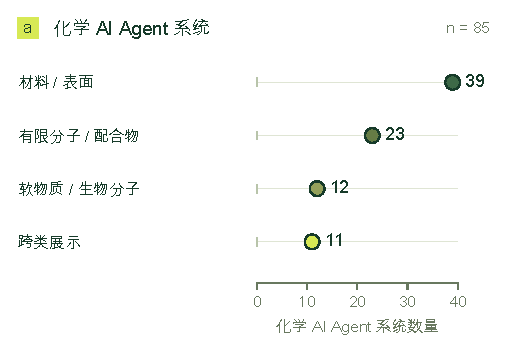
\includegraphics[width=\linewidth]{figures/fig01.pdf}
\caption{85个化学 AI Agent 系统的结构化文献样本：材料/表面39项、有限分子/配合物23项、软物质/生物分子12项、跨类系统11项。}
\label{fig:01}
\end{figure}

Cloudra 按照“智能克制”的设计原则，将几何计算和坐标变换交给确定性算子。最大公共子图（MCS）算法检索分子片段，原子映射与反应中心识别将拓扑连接到后续操作的坐标。测量算子返回键长、键角、二面角与立体特征；操作算子执行片段旋转、平移与过渡态装配。模型指定结构变换目标，检查测量变化，再选择下一构型，从而减少人工对齐端点的需要。

\begin{figure}[tbp]
\centering
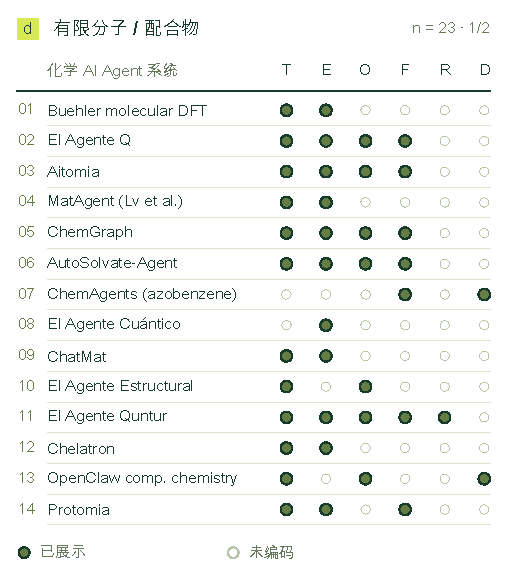
\includegraphics[width=\linewidth]{figures/fig02.pdf}
\caption{有限分子/配合物类已记录的任务（第1/2面板，共23个化学 AI Agent 系统）。T：结构构建/编辑；E：静态能量/性质；O：几何优化；F：振动/热化学；R：显式路径/过渡态；D：分子/量子动力学。实心表示正面证据，空白表示未编码，不代表缺少能力。}
\label{fig:02}
\end{figure}

Cloudra 通过以化学实体为中心的有向无环图（Delivery DAG）组织科学检验。物种与基元步骤为相应计算产物提供归属，步骤记录一阶鞍点和双向 IRC 等检验要求。图将机理主张绑定到用于判断的原始量子化学日志，Supervisor 对照任务契约审核结果，与程序化验收检查共同工作。即使模型提出结束请求，仍缺频率或路径支撑的步骤也保留为未确证。

\begin{figure}[tbp]
\centering
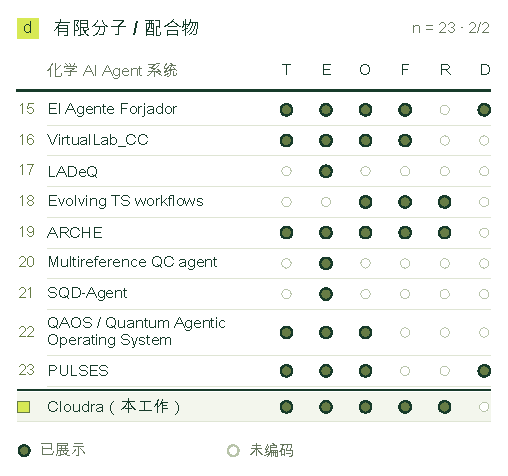
\includegraphics[width=\linewidth]{figures/fig03.pdf}
\caption{有限分子/配合物类化学 AI Agent 系统任务续图（第2/2面板），代码同图~\ref{fig:02}，底端展示 Cloudra（本工作）的能力覆盖。全部85个化学 AI Agent 系统的完整矩阵及逐项来源限制见配套材料。}
\label{fig:03}
\end{figure}

\subsection{主要贡献}

Delivery DAG 将科学检验要求分配给化学物种与基元步骤，并记录尚未满足的要求。检查以量子化学计算产物为依据，使系统能够在研究过程中持续对照物理验收条件判断结束请求。

Cloudra 将 MCS 拓扑映射、位阻图遍历及过渡态片段装配等几何操作实现为确定性程序。语言模型调用这些程序探索化学假设、比较竞争通道并修订计算尝试。

CloudraBench 依据原生计算产物评价图结构覆盖、物理自洽性和定量能垒准确度。50题涵盖基元与多步反应、立体化学及允许方法的适用边界。实验包括四题三次重复的48次运行，以及覆盖50题、四种配置的200次全基准运行。主要比较采用同一模型主干的 Standard，Record 与 Brief-errors 分析证据组织和诊断反馈的作用。
